\section{Brownie Point Nominations}

\begin{frame}{\#1 Figure showing 4 round distinguisher}
  \begin{figure}
    \centering
    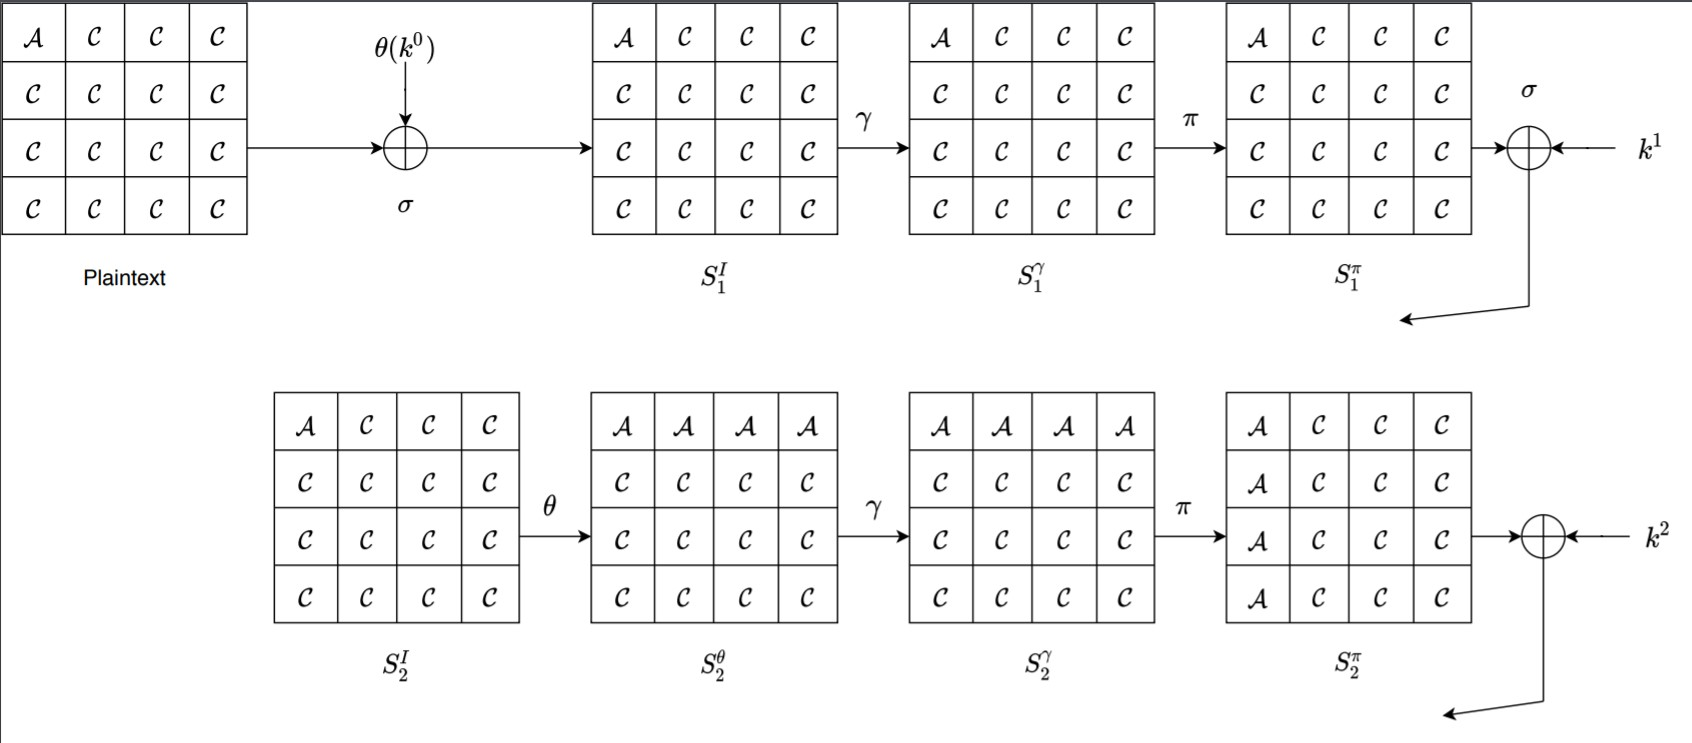
\includegraphics[width=\linewidth]{sq_attack1}
    \caption{Integral attack distinguisher}
  \end{figure}
\end{frame}

\begin{frame}{\#2 Integral Attack Implementation}
  C++ Implementation of 4 round integral attack
\end{frame}

\begin{frame}{\#3 Similarity of Inverse Cipher}
  The SQUARE cipher and it's inverse are very similar. We can use the cipher in place of it's inverse just by replacing $\gamma$ with $\gamma^{-1}$, $\theta$ with $\theta^{-1}$ and keys $k^t$ with $\theta(k^{8-t})$.
\end{frame}